%!TEX root = ../main.tex

\graphicspath{{./figures/chapter3/}}

\chapter{Single-cell segmentation}
\label{ch:chapter3}

\minitoc
\newpage

In this chapter, I review different techniques for nucleus and cell segmentation.
Recently, the solutions proposed to solve this problem have considerably improved, driven by the wave of deep learning models.

After a brief review of the literature in the first part, I describe the methods implemented in \emph{bigfish.segmentation} in a second part.
These methods are published in the paper~\cite{Imbert_fq_2022}:

\begin{center}
	\color{green}
	A. Imbert, W. Ouyang et al. (2022), \textit{FISH-quant v2: a scalable and modular tool for smFISH image analysis}, RNA, pp. $\operatorname{786--795}$, iSSN: $\operatorname{1355--8382, 1469--9001}$.
\end{center}

In a third part, I briefly present two projects for which I have contributed with the objective to boost segmentation efficiency, either by improving the consistency of segmentation masks or by reducing the number of training examples needed.
The former is a preliminary work with incomplete results and the latter was published at the ECCV Bioimage Computing Workshop (BIC)~\cite{Bonte_2022}:

\begin{center}
	\color{green}
	T. Bonte, M. Philbert et al. (2022), \textit{Learning with minimal effort: leveraging in silico labeling for cell and nucleus segmentation}, in 2022 European Conference on Computer Vision (ECCV 2022) Workshop on BioImage Computing.
\end{center}

\section{Segmentation of nuclei and cells in fluorescence microscopy}
\label{sec:segmentation_introduction}

First, I describe the segmentation task that comes in different flavors.
Then, I review different methods that address nucleus and cell segmentation, especially deep learning based models.

\subsection{Computer Vision for cell segmentation}
\label{subsec:segmentation_instance_introduction}

The most useful tasks of Computer Vision in bioimage analysis are classification, object detection and object segmentation.
Classification is concerned with predicting a label for a given input image.
Object detection aims at both classifying and localizing objects inside an image, where localization normally amounts to returning the coordinates of the bounding box of the object.
Of note, object detection is designed to detect several instances of the same object class.
Finally, a segmentation model returns returns a mask for the targeted objects.
If the model does not distinguish between instances of the same object class, it is a semantic segmentation model.
Semantic segmentation resumes to pixel classification, where each individual pixel is classified into object or background (or potentially different foreground classes).
In contrast, the most important segmentation problem in bioimage analysis is instance segmentation, where the model not only distinguishes between foreground and background but also between different objects.
This kind of models is of particular interest for cell and nuclei segmentation, as both cells and nuclei often touch each other.

An example of instance segmentation with nuclei and cells is shown in Figure~\ref{fig:instance_segmentation_example}.
A unique identifier and segmentation mask are returned for every instance.
In Figure~\ref{fig:instance_segmentation_example}, segmentation masks have been postprocessed such that a nucleus has the same identifier as its corresponding cell.

\begin{figure}[]
    \centering
    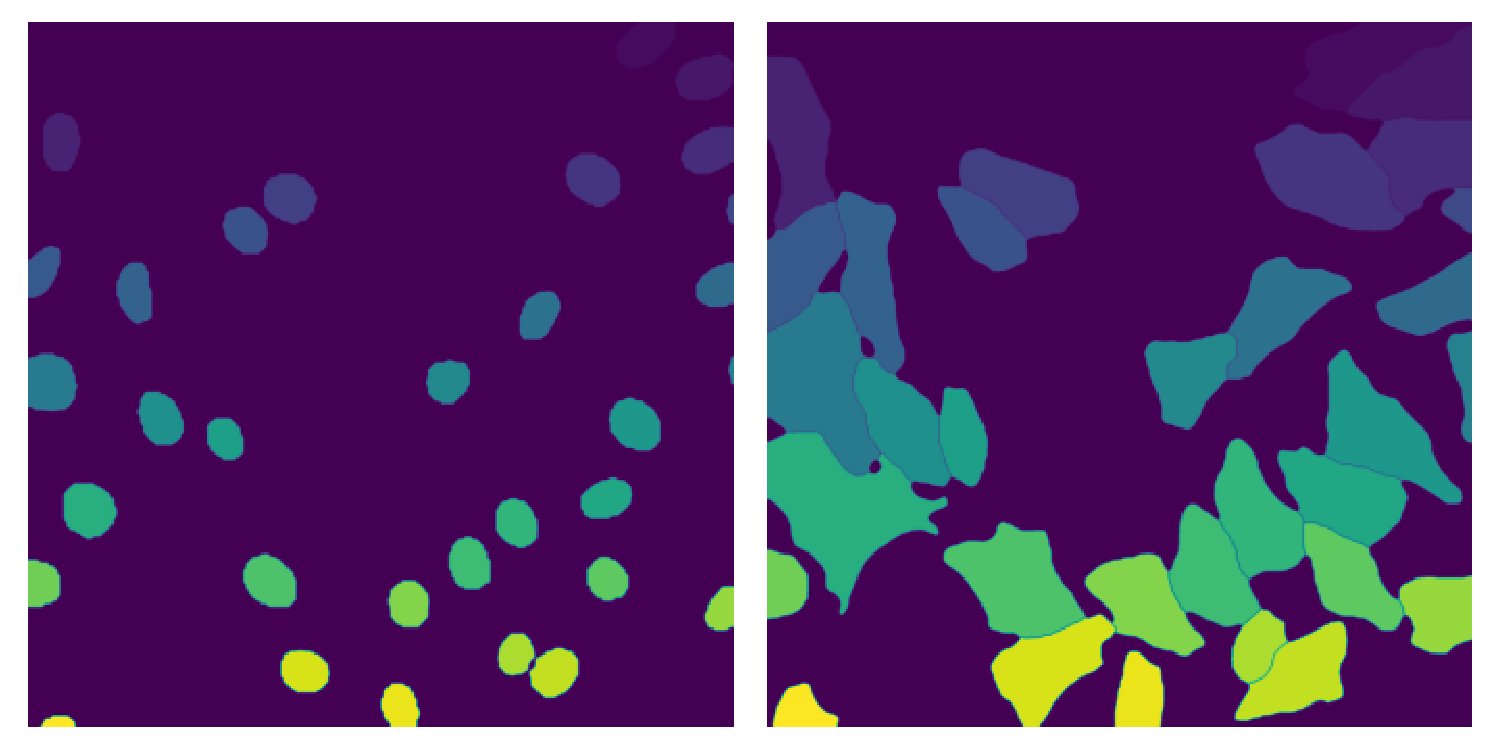
\includegraphics[width=\textwidth]{figures/chapter3/instance_segmentation}
    \caption[Example of instance segmentation]{Example of instance segmentation.
	(\textit{Left}) Nucleus masks.
	(\textit{Right}) Cell masks.
	Every nucleus and cell instance has a different colored mask.
	Plot built with \emph{bigfish}}
    \label{fig:instance_segmentation_example}
\end{figure}

For the rest of the chapter, I only consider 2D segmentation.
Models for 3D segmentation are emerging in the literature, but as manual annotation in 3D is complex and time-consuming, it does not seem an interesting option for our applications.

A specific difficulty with instance segmentation, compared to semantic segmentation, is the need to discriminate between two adjacent instances.
In case of cell segmentation, this is particularly important.
For instance, if we wish to quantify cell shape properties or assess the number of \ac{RNA} inside a cell, it is essential to be able to extract the contours of the cells with high accuracy.

Even though it might be tempting in some applications to omit the cell segmentation step altogether and to classify images of entire cell populations~\cite{Godinez2017}, I believe that cell and nucleus segmentation add great value to the analysis pipelines as they enable one to assign every phenotype or pattern detected in an image to an individual cell.
Segmentation is thus the corner stone of any single-cell analysis.
Instance segmentation is a critical step to capture information at the cell level, especially when the biological mechanism studied exhibits a high intracellular heterogeneity.

\subsection{Related work}
\label{subsec:segmentation_related_work}

\subsubsection{From mathematical morphology\dots}

Fluorescence Microscopy has been specifically designed to provide images, where structures of interest appear with high contrast, while irrelevant structures are invisible.
This can greatly simplify the segmentation task, in particular when objects are isolated and can be easily discriminated from the background, for instance DAPI stained nuclei.
Therefore, a first approach, simple but often successful, is to threshold the image to discriminate foreground from background, and then identify each disconnected mask with a unique identifier to label the objects.
To avoid manual setting of the threshold for each image, automatic methods based on histogram intensity analysis can be exploited, such as Otsu thresholding~\cite{Otsu_1979}.
For clustered nuclei or images with crowded cells, this method does not work and more complex algorithms are needed.

A popular method for segmentation of nuclei and cells is the watershed algorithm~\cite{Beucher1979, Serra1983, Vincent_1991}.
An image is interpreted as a local topography (higher values are peaks and crests, lower values valleys and basins).
There are several variants of this method, but basically the algorithm requires three elements: the starting points from which we flood the image (the markers or seeds; the local minima as default), a relevant topographic representation of our image where the boundaries of the object have higher pixel values, and optionally a binary mask limiting the flooding area (the mask).
The Watershed algorithm simulates a flooding of the surface where pixels are subsequently added to the extending seed regions in such a way that pixels with lower value are always processed first.
Object boundaries are found where the extending seed regions meet.

This is an attractive strategy for cell segmentation~\cite{Wahlby2002}.
We can use the previously detected nuclei as seeds, which guarantees that all detected cells will have one nucleus, which is inside the cellular region, by design of the algorithm.
Furthermore, there are numerous possibilities to construct an image to be flooded, depending on the employed marker: either the image itself (e.g.~in case of a membrane marker) is used, a gradient image (e.g.~in case of a cytoplasmic marker with different expression levels) or the distance map of a binary image (which was the original idea).
Unfortunately, if we miss some nuclei at the beginning, the error impacts the rest of the computational pipeline.
Not only do we miss potentially interesting cells, but we also wrongly assign cytoplasmic regions to cells where they do not belong.
For this reason, it is important that the nuclei detection returns accurate results.

Many other segmentation methods have been proposed in the computer vision literature.
Superpixel approaches, for instance, partition the image into multiple homogeneous regions with enforced compactness~\cite{Ren_2003}.
Low-level segmentation algorithms such as watershed itself can help form these regions by clustering pixels together~\cite{Machairas_2014}.
These superpixel can then be merged by heuristics or graph-based approaches.
The segmentation task can also be addressed from the boundaries point of view.
Active contour models (or snakes) rely on energy minimization techniques to deform a spline curve until it delineates the object outline~\cite{kass_snakes_1988}.
The advantage of this method is that a priori knowledge on the cell or nuclear geometry can be incorporated into the segmentation algorithm~\cite{Dufour2005}.

For most segmentation benchmarks, these methods have been outdated in recent years, with the emergence of deep learning models trained on large and diverse datasets.
However, mathematical morphology methods remain relevant for some use cases.
Most importantly, these traditional methods do not require manual annotation, which is often a bottleneck for medical or biological image segmentation.
Eventually, such algorithms can also inspire new learning-based models, like Deep watershed model that predicts a watershed energy map before extracting object instances from it~\cite{Bai_2017_CVPR}.

\subsubsection{\dots to deep learning models}

% recent successes
Deep learning literature for image segmentation has provided several powerful and consistent models.
Mostly based on \ac{CNN}, they have dramatically boosted computer vision applications.
This trend keeps influencing bioimage informatics as well.

% U-Net
One of the seminal neural networks proposed for biomedical segmentation is U-Net~\cite{Ronneberger_2015}.
The network has a U-shaped architecture with an encoder and a decoder.
The former combines convolutional layers, non linear activation functions (ReLU) and max pooling operations to reduce spatial information and expand feature information.
The latter includes upsampling layers to return an output segmentation map that is postprocessed in order to build a (semantic) segmentation mask.
This architecture is now a classic and it is vastly reused by more recent work like StarDist~\cite{schmidt2018}, which is trained to predict star-convex polygons for each nucleus or cell instance.

% importance of dataset
One the main limitations of deep learning methods in general is the need for a large amount of annotated images to train the models.
For image classification, this problem was addressed by the publication of large annotated dataset of natural images like ImageNet~\cite{Deng_2009} or COCO dataset~\cite{Lin_2014}.
Following this example, recent publications in biomedical segmentation include sometimes both a trained model and a release of an important dataset with segmented nuclei or cells.
For example, the research community benefits from an online challenge organized in 2018 about nucleus segmentation: the 2018 Data Science Bowl\footnote{\url{https://www.kaggle.com/c/data-science-bowl-2018}}.
This competition includes a large collection of images with different modalities (histopathology, fluorescence microscopy).

% NucleAIzer
NucleAIzer~\cite{hollandi_nucleaizer_2020} proposes a model inspired by the winning solutions of the 2018 challenge and trained on the released dataset.
It combines Mask R-CNN~\cite{He_2017_ICCV} and U-Net.
Post competition, it outperforms all the submitted methods of the competition.

% Cellpose
Cellpose~\cite{stringer_cellpose_2021} proposes a U-Net based model for nucleus and cell segmentation.
The network is trained to predict horizontal and vertical gradients of the topological cell map.
These gradients form a vector field where each pixel ''belonging to a given cell can be routed to its center''.
By grouping pixels converging to the same regions, individual instances can be identified.
Most importantly, authors have collected and manually annotated 608 cell images with various modalities.
Currently, this solution appears to be one of the most efficient, even though it remains unclear whether this is attributed to the dataset, the architecture or the formulation of the prediction task.
The authors have extended their method by training it with several specialized datasets like TissueNet~\cite{Greenwald_2022} or bacteria images~\cite{cutler_omnipose_2022}.

% adaptated from natural image model
Another important factor for progress in segmentation is the state of the literature on natural image segmentation.
Indeed, several methods published for biomedical segmentations are inspired from a previous model trained on natural images.
For example, NucleAIzer reuses Mask R-CNN, a \ac{CNN} that combines ideas from object detection and image segmentation.
Mask R-CNN suggests regions of interest, detects object instances within these regions and performs instance segmentation with a fully convolutional branch.
When released in 2017, the model was state-of-the-art on the COCO dataset.
This relationship can also be observed with EmbedSeg~\cite{Lalit_2021} directly inspired by~\cite{Neven_2019_CVPR}.

\section{Segmentation models}
\label{sec:segmentation_nuc_cell}

In this section, I first describe a dataset I have annotated in order to train deep learning segmentation models.
Then, I detail the solutions implemented in \emph{bigfish.segmentation} to segment both nuclei and cells.
In addition, several postprocessing functions are presented to refine any segmentation results.

\subsection{A new multichannel dataset}
\label{subsec:segmentation_data}

\begin{figure}[]
	\centering
	\minipage{0.5\textwidth}
		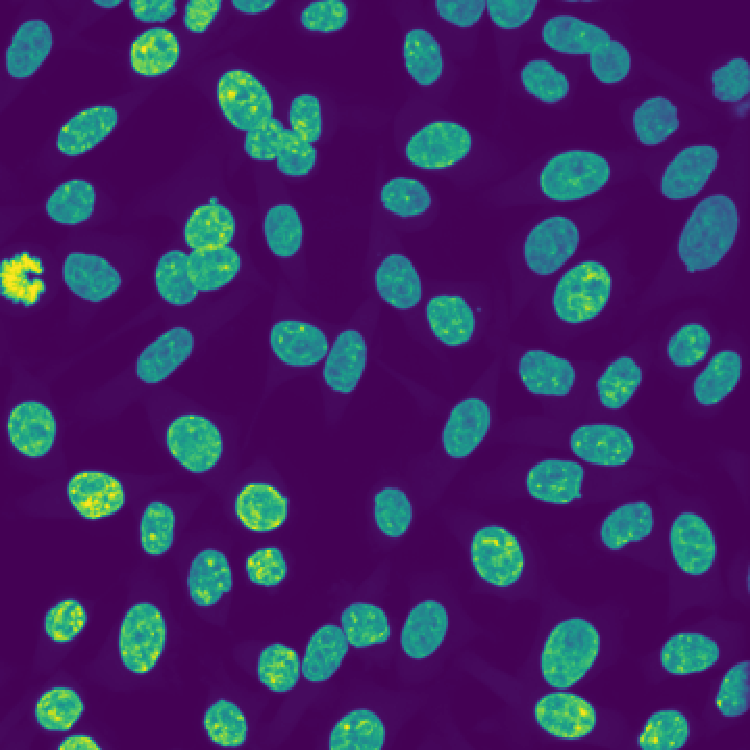
\includegraphics[width=0.95\linewidth]{figures/chapter3/dapi_BICD2}
		\subcaption{DAPI channel}
		\vfill
		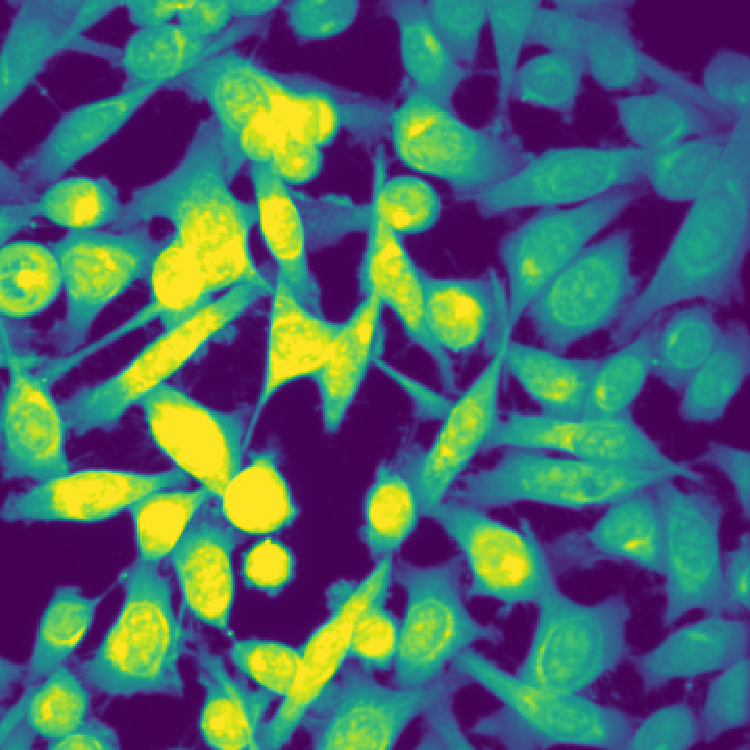
\includegraphics[width=0.95\linewidth]{figures/chapter3/cellmask_BICD2}
		\subcaption{CellMask\textsuperscript{\texttrademark} channel}
	\endminipage\hfill
	\minipage{0.5\textwidth}
		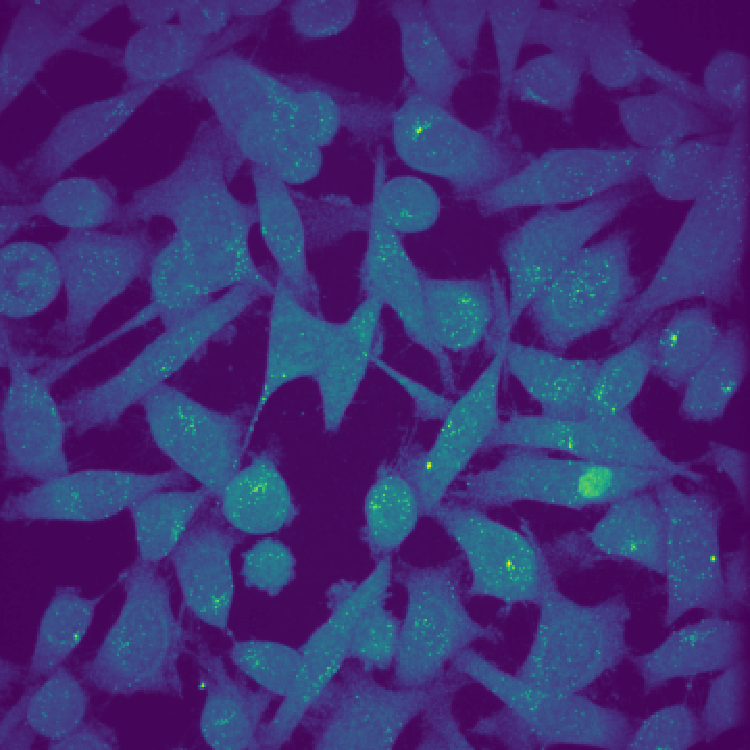
\includegraphics[width=0.95\linewidth]{figures/chapter3/smfish_BICD2}
		\subcaption{smFISH channel}
		\vfill
		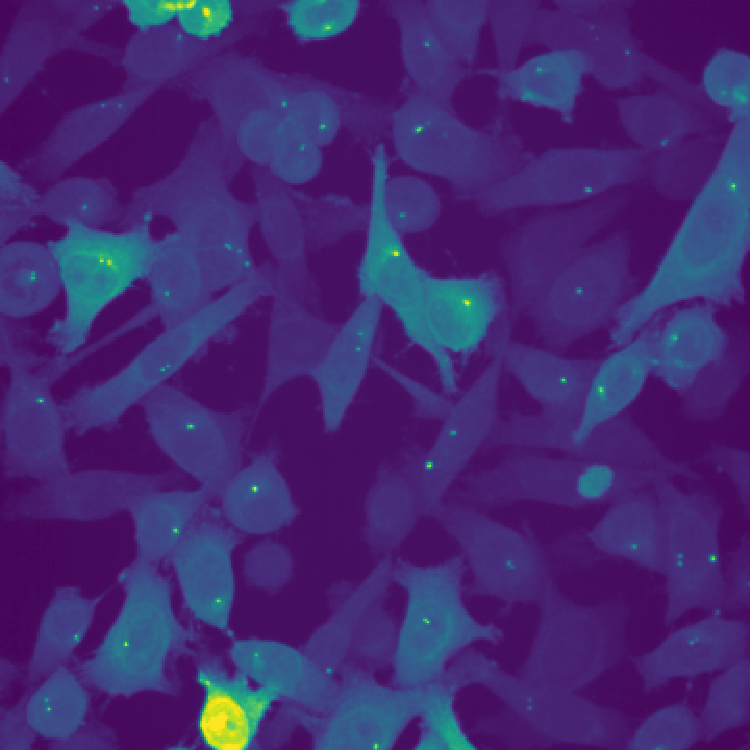
\includegraphics[width=0.95\linewidth]{figures/chapter3/gfp_BICD2}
		\subcaption{GFP channel}
	\endminipage
	\caption[Segmentation dataset]{Multichannel annotated images for nucleus and cell segmentation.
	Images are projected in 2D.
	Plot built with \emph{bigfish}}
	\label{fig:annotated_dataset_segmentation}
\end{figure}

I use the 4-channel images from one of our applications~\cite{safieddine_choreography_2021} presented in Chapter~\ref{ch:chapter5} to build an annotated dataset for the segmentation task.
I randomly sample 180 \ac{FoV}s.
Each image includes one channel adapted for nucleus segmentation (DAPI) and three channels adapted for cell segmentation (\ac{smFISH}, CellMask\textsuperscript{\texttrademark} and a \ac{GFP} marker for the centrosome).
An example of these images is illustrated in Figure~\ref{fig:annotated_dataset_segmentation}.
The ground truth annotation is obtained in two steps: I pre-segment nuclei and cell with a Cellpose model~\cite{stringer_cellpose_2021}, then I manually correct these predictions.
In total, 4,026 cell instances are segmented, with their relative nucleus.

The initial goal for this dataset is to train segmentation models and perform some experiments to evaluate their consistency.
In particular, I am interested in:

\begin{enumerate}
	\setlength\itemsep{0.1em}
	\item Consistency between nucleus and cell segmentation, two tasks often performed independently.
	The dataset is annotated such that each instance has a nucleus and a cell mask, matching together.
	This also enables a potential joint training of nucleus and cell segmentation.
	\item Input heterogeneity.
	Here, the cell related channels come from three different modalities of acquisition.
	A priori, a model trained on CellMask\textsuperscript{\texttrademark} should be more efficient, but because this label is not always available in an experimental setup, it is interesting to train models robust enough to identify cells from different channels.
\end{enumerate}

\subsection{Nucleus segmentation}
\label{subsec:segmentation_nuc}

Nucleus segmentation is usually the first task in cellular image analysis, applied on a DAPI channel for example.
An error during this step can propagate to the rest of the analysis, if the cell segmentation and identification is based on an initial nucleus segmentation.
In particular, it is important to avoid missed nuclei and nuclei that are split in several parts.
In \emph{bigfish}, I have implemented simple thresholding techniques, and a simple deep learning model for nucleus segmentation.

\subsubsection{A 3-class deep learning model}

The model is described in~\cite{Imbert_fq_2022}.
It uses an encoder-decoder architecture like U-Net~\cite{Ronneberger_unet}, with 4 downsampling stages.
In total, the spatial resolution of the input image is divided by 16 at the bottom of the model.
For each stage, I implement residual blocks, mimicking Cellpose model~\cite{stringer_cellpose_2021}.
Lastly, the upsampling stage is implemented following deconvolution techniques from~\cite{odena2016deconvolution} to prevent any checkerboard artifacts.

The nucleus segmentation problem is address like a pixel-wise classification problem with three classes: background, foreground and nuclear boundary.
My model assigns one of these three classes to each pixel.
The returned final mask is the foreground predicted surface, postprocessed with a dilation of 1 pixel.
This model is trained on the DAPI channel from the annotated dataset presented in~\ref{subsec:segmentation_data}, with a categorical cross-entropy loss.\\

\begin{minipage}{0.9\textwidth}
\begin{lstlisting}[language=Python]
import bigfish.segmentation as segmentation

# load pretrained model
model_nuc = segmentation.unet_3_classes_nuc()

# instance segmentation
nuc_label = segmentation.apply_unet_3_classes(
    model=model_nuc,
	image=image_nuc,
	target_size=256,
	test_time_augmentation=True)
\end{lstlisting}
\end{minipage}

\subsubsection{Multiple rounds of segmentation}

Despite overall good results, I noted that some (dim) nuclei are missed altogether by the algorithm.
In \emph{bigfish.segmentation}, I implement a method to remove segmented nuclei from a DAPI channel, in order to perform a second round of segmentation.
This strategy is useful if the employed segmentation method misses too many nuclei at first try.
Such failures can be due to a heterogeneous DAPI signal between cells, to the presence of adjacent nuclei or instances with unusual shape.

Removal of segmented nuclei is based on morphological reconstruction and based on the following steps:
\begin{enumerate}
	\setlength\itemsep{0.1em}
	\item The binary mask of the segmented nuclei is dilated.
	\item From the original DAPI image $f$, an image $g$ is generated where all pixels outside of the dilated mask are set to zero.
	This includes the background and the potentially missed nuclei.
	\item A morphological reconstruction $R^{\delta}_f(g)$ by dilation~\cite{Serra1983, Soille2003, Robinson_2004} of $g$ under $f$ allows to reconstruct the background signal, but not the missed nuclei.
	As a consequence the reconstructed image only differs from the original one where the nuclei have been missed in the first place.
	\item The residue image $\Delta = f - R^{\delta}_f(g)$ thus contains the missed nuclei and can then be thresholded to complete the detected nuclei.
\end{enumerate}

\noindent
Finally, after a second round of segmentation, the two obtained nucleus segmentation masks can be merged together.
Surprisingly, repetitive application of the same segmentation model seems to help improving the final segmentation.
In particular, I applied this technique in~\cite{CHOUAIB_2020}.\\

\begin{minipage}{0.9\textwidth}
\begin{lstlisting}[language=Python]
import bigfish.segmentation as segmentation

# first attempt of segmentation (with missing nuclei)
#nuc_label_1 = model(nuc_image)

# remove segmented nuclei
remaining_nuc_image = segmentation.remove_segmented_nuc(
	image=nuc_image,
	nuc_mask=nuc_label_1)

# second attempt of segmentation
#nuc_label_2 = model(remaining_nuc_image)

# merge nucleus labels
nuc_label = segmentation.merge_labels(nuc_label_1, nuc_label_2)
\end{lstlisting}
\end{minipage}

\subsection{Cell segmentation}
\label{subsec:segmentation_cell}

Cell segmentation is often more difficult.
It can involve images with cluttered cells, fluorescent labels with different quality or labels not initially designed to visualize the cytoplasm (for example, the \ac{smFISH} channel).
In addition, cells can exhibit more diversity in their morphological shapes than nuclei, and a successful method with HeLa cells could fail in other cell lines or bacteria images.

A watershed algorithm is available in \emph{bigfish.segmentation} to discriminate adjacent cells, where 
a previous nucleus segmentation mask is used as marker.
The Watershed transform is applied to the input channel, potentially regularized with the distance map from nuclei (an image where each pixel takes the distance to the nucleus).

\subsubsection{A revisited deep watershed model}

I also implement a deep learning solution for cell segmentation, inspired by Deep Watershed~\cite{Bai_2017_CVPR} and the use of distance maps for nucleus segmentation~\cite{Naylor_2019}.
Two models are tested, with the same backbone architecture previously presented for nucleus segmentation: an encoder-decoder convolutional neural network with residual blocks.

A first model uses only one input image with cell information (in my case, CellMask\textsuperscript{\texttrademark}, \ac{smFISH} or \ac{GFP}).
This model predicts two outputs: a binary mask of cell surface (like in semantic segmentation tasks) and a distance map to cell edges.
The idea is that forcing the network to predict a distance map will ultimately push it to learn the specific local patterns indicating the position of the plasma membrane, a pre-requirement for instance segmentation.
These outcomes are then used in a watershed algorithm with the segmented nuclei as seeds in order to return a segmentation mask for every cell instance.
The model is trained with a combined loss averaging a binary cross-entropy loss for the surface prediction and a mean absolute loss for the distance map.

A second model uses two channels as input images, one for the nuclei and one for the cells.
In addition to the two previous output images, it predicts a third output: a distance map to nucleus edges.
Cell instances are obtained with the same strategy as above, namely by application of a watershed algorithm  applied on the predicted distance map with the segmented nuclei as seeds.
The idea is to add input information about the nuclei and to force the model to take it into account by returning a nucleus related prediction.
I hypothesized that this would make cell segmentation more accurate, as more local cell and nuclei features are predicted.
In \emph{bigfish.segmentation} this second model is implemented, with a double input strategy.\\

\begin{minipage}{0.9\textwidth}
\begin{lstlisting}[language=Python]
import bigfish.segmentation as segmentation

# load pretrained model
model_cell = segmentation.unet_distance_edge_double()

# instance segmentation
cell_label = segmentation.apply_unet_distance_double(
    model=model_cell,
    nuc=image_nuc,
    cell=image_cell,
    nuc_label=nuc_label,
    target_size=256,
	test_time_augmentation=True)
\end{lstlisting}
\end{minipage}

\subsubsection{Segmentation evaluation}

The main advantages of the available deep learning models in \emph{bigfish.segmentation} is to offer an efficient in-house segmentation solution, without the need to use another API, package or framework.
It is fast to apply and can be a relevant first solution to try.
However, for more challenging segmentation problems, FISH-quant v2 still enables the use of external resources like Cellpose or StarDist.

Both nucleus and cell segmentation models are trained with Adam optimizer~\cite{Diederik_2015} until validation loss does not improve anymore.
Performance is assessed with the mean Average Precision.
The \ac{IoU} score is computed for each pair of predicted and ground truth instances (whose value ranges between 0 and 1).
Prediction matches the ground truth if the \ac{IoU} is above a specific threshold.
Therefore, for a given threshold, I can compute True Positives (instances matched correctly), False Positives (predicted instances matching nothing), False Negatives (ground truth instances missed) and the \ac{AP} score such that:

\begin{equation}
	{\displaystyle \operatorname{AP} = \frac{\operatorname{TP}}{\operatorname{TP} + \operatorname{FP} + \operatorname{FN}}}
\end{equation}

The mean Average Precision is the average of the \ac{AP} score for different \ac{IoU} thresholds between 0.5 and 0.95.
A higher value indicates a better agreement between prediction and ground truth instances.

Results for my deep learning implementations are shown in Table~\ref{table:segmentation_results}.
Evaluation is performed on the multichannel dataset extracted from~\cite{safieddine_choreography_2021}.
As expected, best results for cell segmentation are obtained with CellMask\textsuperscript{\texttrademark} input, while \ac{smFISH} and \ac{GFP} channels yielded similar \ac{AP} scores.
Interestingly, the addition of nucleus information in input slightly improves cell segmentation results for the \ac{smFISH} and \ac{GFP} channels.

\begin{table}[]
	\centering
	\begin{tabular}{| c | c | c | c | c |}
		\hline
		Model & DAPI & CellMask\textsuperscript{\texttrademark} & smFISH & GFP\\
		\hline
		3-class U-Net & \textbf{0.6} & - & - & -\\
		Distance map U-Net & - & \textbf{0.66} & 0.59 & 0.58\\
		Distance map U-Net (double input) & - & 0.65 & \textbf{0.63} & \textbf{0.62}\\
		\hline
	\end{tabular}
	\caption[Segmentation results]{Segmentation results for different input channels.
	Computed score is the mean Average Precision, the higher, the better.
	Best models are bold.
	Evaluation is performed over 19 images}
	\label{table:segmentation_results}
\end{table}

\subsubsection{Postprocessing and refinement}

Regardless of the segmentation method applied, \emph{bigfish.segmentation} includes different methods to clean and refine the segmentation masks.
The most simple operations consist in smoothing the mask boundaries with a median filter, removing the small disjoint masks or filling holes within the segmented areas.

It can also be useful to separate the labeled instances in the labelled image $y$.
For this, I can simply calculate the morphological gradient $\rho = \delta(y) - \varepsilon(y)$ (the difference between the dilation $\delta$ and the erosion $\varepsilon$ of a given image) and then separate the instance by setting $y(x) = 0, \: \forall x: \rho(x) > 0$.
An example of such refined results is illustrated in Figure~\ref{fig:instance_segmentation_example}.

Lastly, if nucleus and cell segmentation maps have been generated by independent algorithms, they need to be matched.
For this, I also propose a small helper function in \emph{bigfish.segmentation}.\\

\begin{minipage}{0.9\textwidth}
\begin{lstlisting}[language=Python]
import bigfish.segmentation as segmentation
import bigfish.multistack as multistack

nuc_label = segmentation.clean_segmentation(
	nuc_label=nuc_label,
	delimit_instance=True)
cell_label = segmentation.clean_segmentation(
	cell_label=cell_label,
	smoothness=7,
	delimit_instance=True)
nuc_label, cell_label = multistack.match_nuc_cell(
	nuc_label=nuc_label,
	cell_label=cell_label,
	single_nuc=False,
	cell_alone=True)
\end{lstlisting}
\end{minipage}

\section{Improving cell segmentation}
\label{sec:segmentation_improvements}

I have contributed to two projects with the aim to improve specific aspects of biomedical segmentation.
The first project consisted in developing a deep learning version of the active contour algorithm.
However, this work is not finished and it yielded incomplete results so far, so here I only present the main idea.
The second project aimed at leveraging in-silico labeling in order to pre-train segmentation models without manual annotation and resulted in a publication~\cite{Bonte_2022}.

\begin{figure}[]
    \centering
    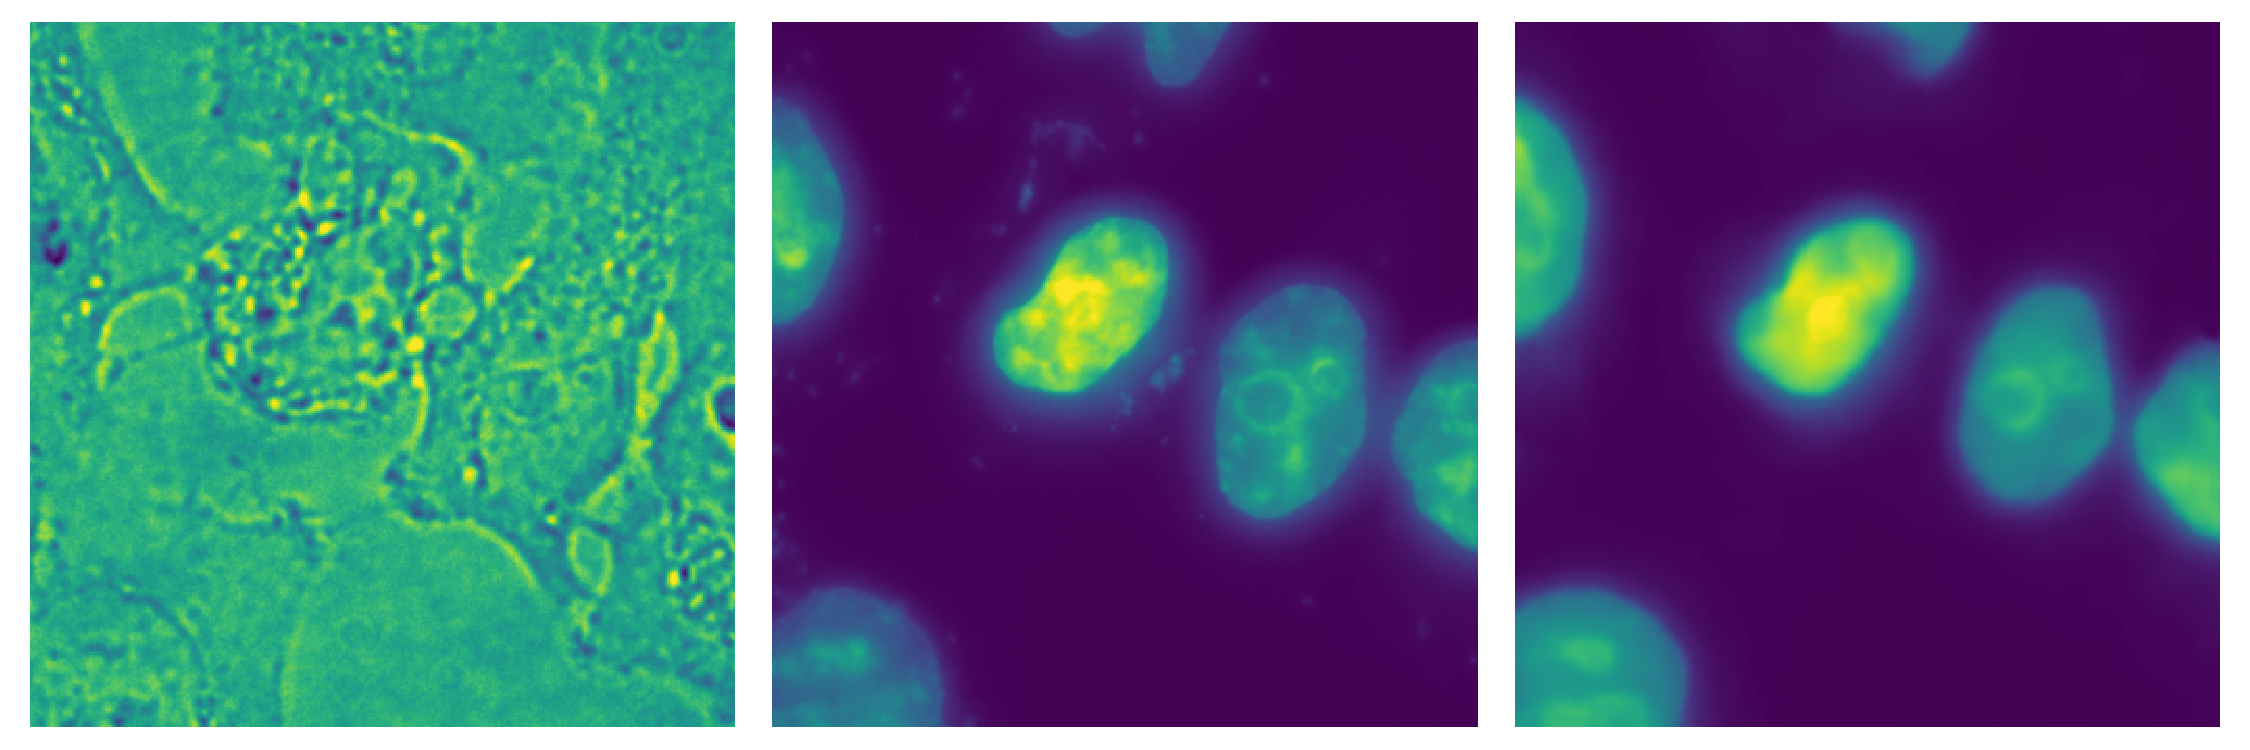
\includegraphics[width=\textwidth]{figures/chapter3/insilico_prediction}
    \caption[Example of in silico labeling]{Example of in silico labeling, from~\cite{Bonte_2022}.
	(\textit{Left}) Bright-field input image.
	(\textit{Center}) Ground truth DAPI channel.
	(\textit{Right}) Predicted DAPI}
    \label{fig:example_insilico}
\end{figure}

\subsection{Snake-like model}
\label{subsec:segmentation_snake}

This project tries to address potential inconsistencies between nucleus and cell segmentation when these two tasks are performed independently.
Sometimes the cell is correctly segmented, but not the nucleus, sometimes it is the opposite.
If I cannot match a nucleus with a cell, the whole instance is discarded.
In addition, nucleus is often far easier to segment than the cell.

The idea is to propagate or extend the cell outline from the nuclear region, which would perfectly solve this problem of inconsistency.
The popular watershed approach does this, but it has a number of well-known limitations in the presence of strongly anisotropic cells and noisy boundaries (leakage).

Inspired by active contour models, the goal is to deform a spline curve around cell instance, but instead of solving an energy minimization problem a neural network would predict the deformation of the polygon.
Such method has already been proposed for natural image segmentation like Deep Snake~\cite{Peng_2020_CVPR} or DANCE~\cite{Liu_2021}.
However, these models need to first detect the candidate object instance and then initialize the deformable polygon from the detected bounding box.
Their entire pipeline relies on the performance of a detection model.
In my case, the cell outline would be initialized from the nucleus outline (much easier to segment), before being iteratively distorted by a fully convolutional network.
Even though the method seemed appealing at first sight, I did not obtain convincing results.

\subsection{In silico pre-training}
\label{subsec:segmentation_insilico}

In a joint work with a master student and another PhD student, we aimed at leveraging \ac{ISL} task to pre-train segmentation model and mitigate the need for annotated training images.
\ac{ISL} consists in predicting fluorescent labels from bright-field or transmitted-light images~\cite{christiansen_silico_2018, ounkomol_label_free_2018}.
The idea is to replace some fluorescence microscopy channels by their predictions (illustrated in Figure~\ref{fig:example_insilico}), in order to free channels for other analyses.

In~\cite{Bonte_2022}, we use the same model to perform \ac{ISL} and segmentation.
It is based on a U-Net architecture, with a DenseNet encoder branch~\cite{Huang_2017_CVPR}.
The first training on \ac{ISL} makes the model learn intermediate visual representations of the cell.
We speculate that these learned features are relevant for the segmentation task.
In this case, the following segmentation training should be more efficient.

In Figure~\ref{fig:results_insilico} we compare the \ac{IoU} score of the trained models for different training set size.
A second model pre-trained with a natural image classification task (from ImageNet~\cite{Deng_2009}) is also displayed for comparison purpose.
The difference in terms of pre-training vanishes when the size of the training set increases.
However, pre-training a segmentation model with \ac{ISL} clearly compensates a low number of training images.

\begin{figure}[]
    \centering
    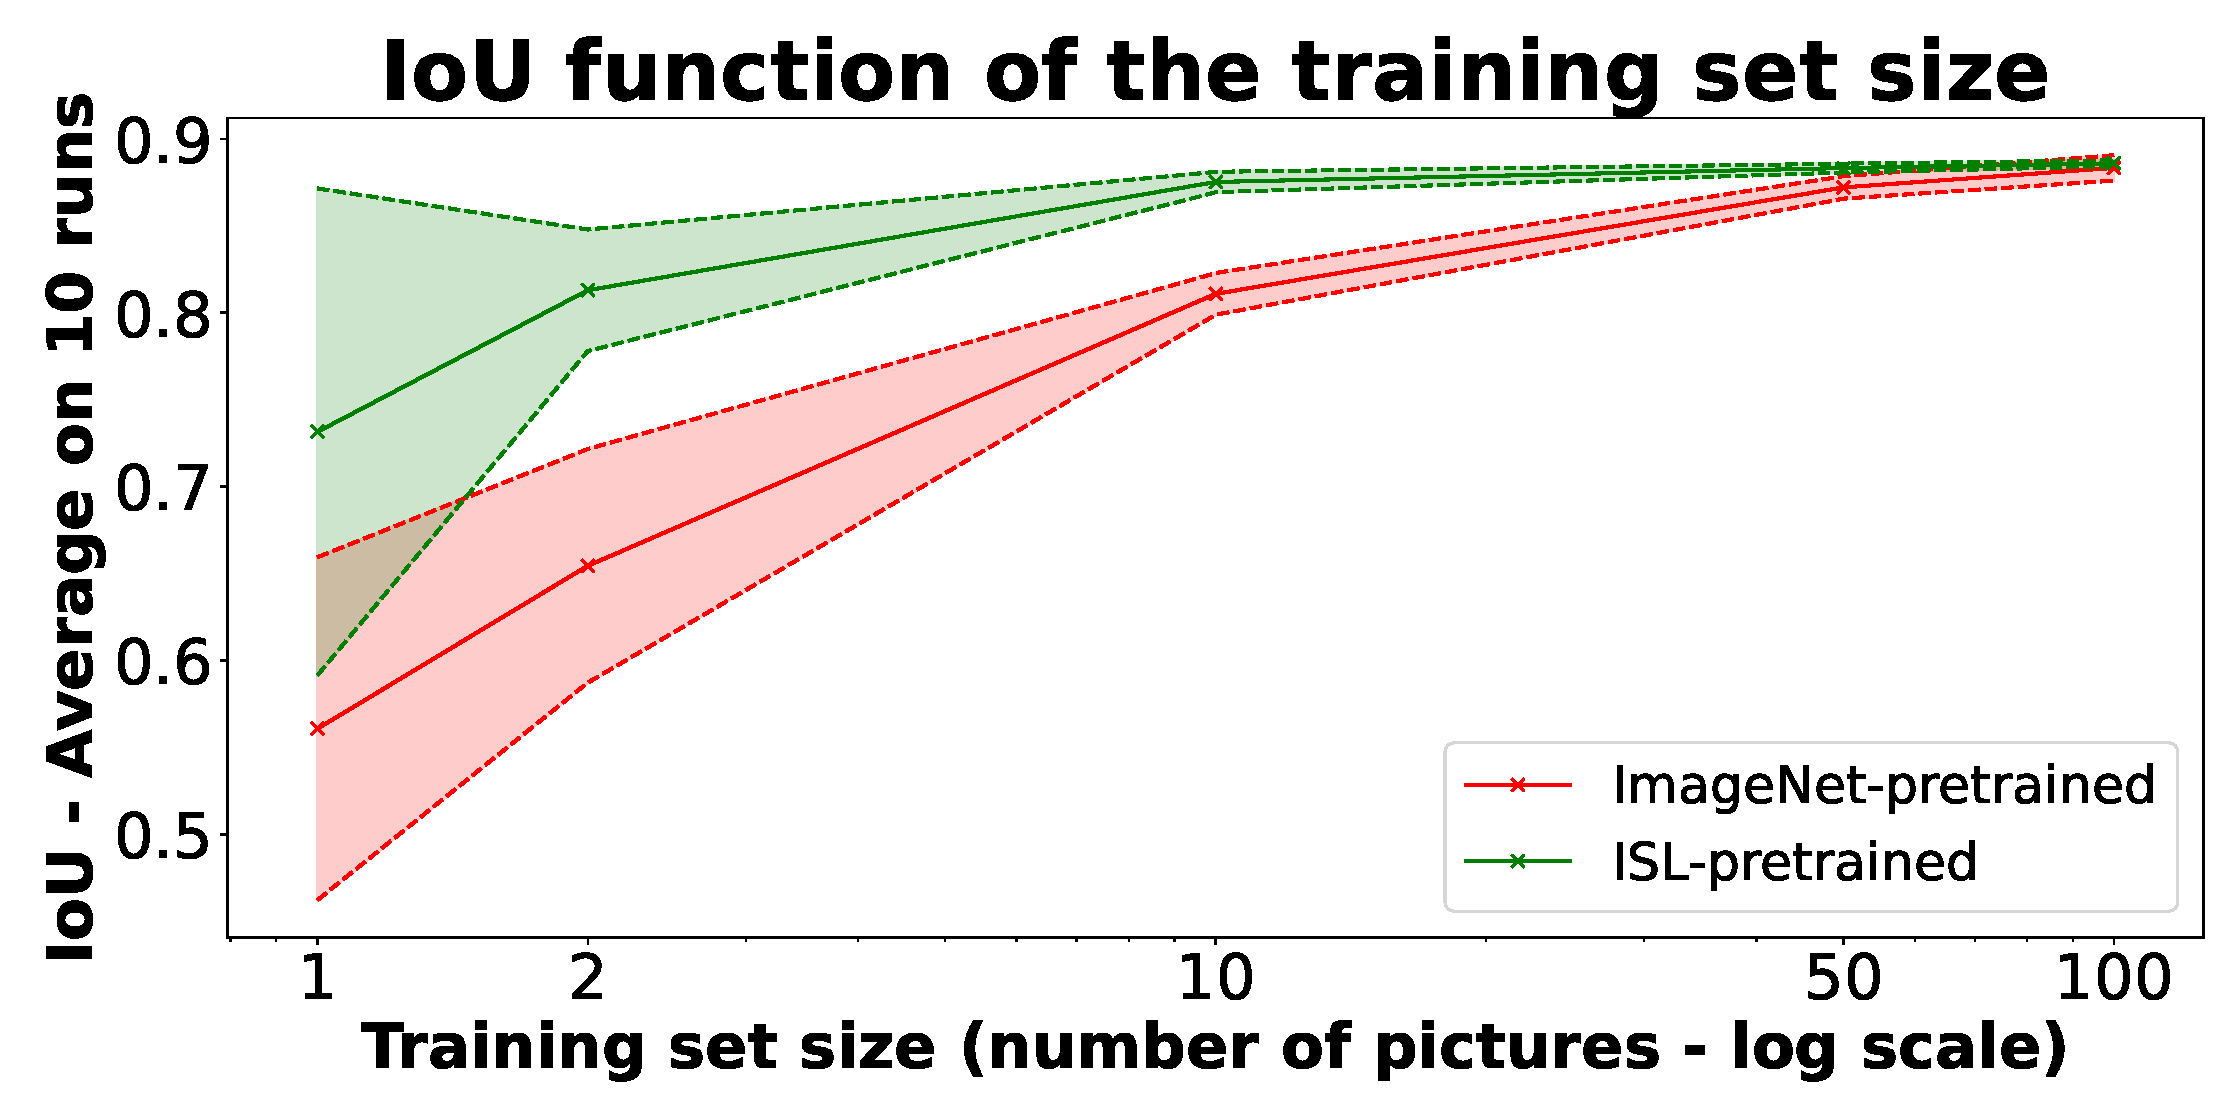
\includegraphics[width=\textwidth]{figures/chapter3/insilico_training_size}
    \caption[Results of in silico pre-training]{Results of in silico pre-training for a nucleus segmentation task, from~\cite{Bonte_2022}.
	IoU score for different training set size (the higher the better).
	Segmentation model with in silico pre-training (\textit{green}) is more efficient in low training dataset regime than model with ImageNet pre-training (\textit{red})}
    \label{fig:results_insilico}
\end{figure}

\section{Conclusion}
\label{sec:segmentation_conclusion}

This chapter details the different algorithms available in \emph{bigfish.segmentation} subpackage to segment nuclei and cells from fluorescent microscopy images.
The main interest of these methods is to propose in-house segmentation solutions, easy to use in a few lines of code, and therefore complete the quantitative pipeline defined in FISH-quant.
Yet, the research community is quite dynamic concerning biomedical segmentation.
A lot of publications are released every year, with new datasets and improved techniques.
Beyond developing a potential state-of-the-art model (which would be surpassed a few months later), the ability to easily integrate results from external resources is essential for FISH-quant.
To this end, postprocessing methods are also implemented to format and refine segmentation masks.

Even if the segmentation has not been my main axis of research, I have explored some methods to alleviate limitations observed in cell segmentation.
During my PhD I have mainly worked with multichannel images considering both nuclei and cells.
For this reason, the consistency between nucleus and cell segmentation is critical.
Such consistency can be directly enforced by the way an algorithm works, like in a watershed transform, or learned through a specific training strategy.
Additionally, the need for a large amount of annotated images is still a hot topic in deep learning research.
The use of in silico techniques to pre-train models seems to mitigate this limitation.
